\chapter{Miscellaneous}

\section{C-like Include Script}

Currently F2J does not support module system, so that the whole program must be written in one file. But in practice, when the program has over 1000 lines, it would be very hard to manage and debug. In this project, the file that contains all test cases of the monadic parser has over 4000 lines of F2J code.

It would be better if just separate those codes into different files and then combine them together before compile. To achieve that goal, we have a script \texttt{include.py} in Python to perform C-like include mechanism of the FParser project (monadic parser combinators).

The script will try to find a special block comment, which starts with \texttt{\{-\#} and ends with \texttt{\#-\}}, and then find a keyword \texttt{INCLUDE} in the block with the file name to be included. For example

\begin{lstlisting}
{-#
    INCLUDE "parser.sf"
    INCLUDE "test.sf"
#-}
\end{lstlisting}

When process this file with \texttt{include.py}, it will search for the special block comment and get the statements \texttt{INCLUDE "parser.sf"} and \texttt{INCLUDE "test.sf"}. And then, it will find the \texttt{parser.sf} and \texttt{test.sf} files in the search path, read them and analysis their include statements recusively. After that, paste the combined files in place of the include statements with the rest of the file contents in the target file.

Because the special block comments are valid F2J comments, so that they will be ignored when compiling.

\section{Test Framework}

If the project is small, then writing and running tests are easy. But when your code grows large, tests become a large code base and become hard to manage and modify.

So we use F2J to write a simple test framework, supporting test functions, test suites and assert functions.

The most basic definitions are in \texttt{testfx.sf} of the FParser project (monadic parser combinators).

Test function is a record, which contains a name and a function to run the test.

\begin{lstlisting}
type TestFn = {
    name : String,
    fn   : Unit -> Bool
};
\end{lstlisting}

If test succeeded, the function should return \texttt{True}, \texttt{False} otherwise.

For test suite, it is a collection of \texttt{TestFn} with name.

\begin{lstlisting}
type TestSuite = {
    name : String,
    fns  : PList[TestFn]
};
\end{lstlisting}

Here is a simple example to run tests.

\begin{lstlisting}
let testFJExprVariable : TestFn = {
    name = "Test Variable a",
    fn   = \(__ : Unit) -> {
        assertParseStringResult[FJExpr]
            fjExprEq
            fjExprToString
            (FJVariable "a")
            fjExpr
            "a"
    }
};

let testFJParserSuite : TestSuite = {
    name = "Test Feather Weight Java parser",
    fns  = testFJExprVariable
                +>[TestFn] (Nil[TestFn])
};

let parserTestSuites : PList[TestSuite] =
    testFJParserSuite
        +>[TestSuite] (Nil[TestSuite]);

runTestSuites parserTestSuites;
\end{lstlisting}

The function \texttt{runTestSuites} is a helper function for running a list of test suites.

The function \texttt{assertParseStringResult} is a helper function, which will judge whether the first parse result is equal to the provided one, it will also prints the expected and actual parse outputs to the screen.

An example in Figure \ref{fig:monadic_runalltests} shows how the test framework runs.

\begin{figure}[h!]
    \centering
    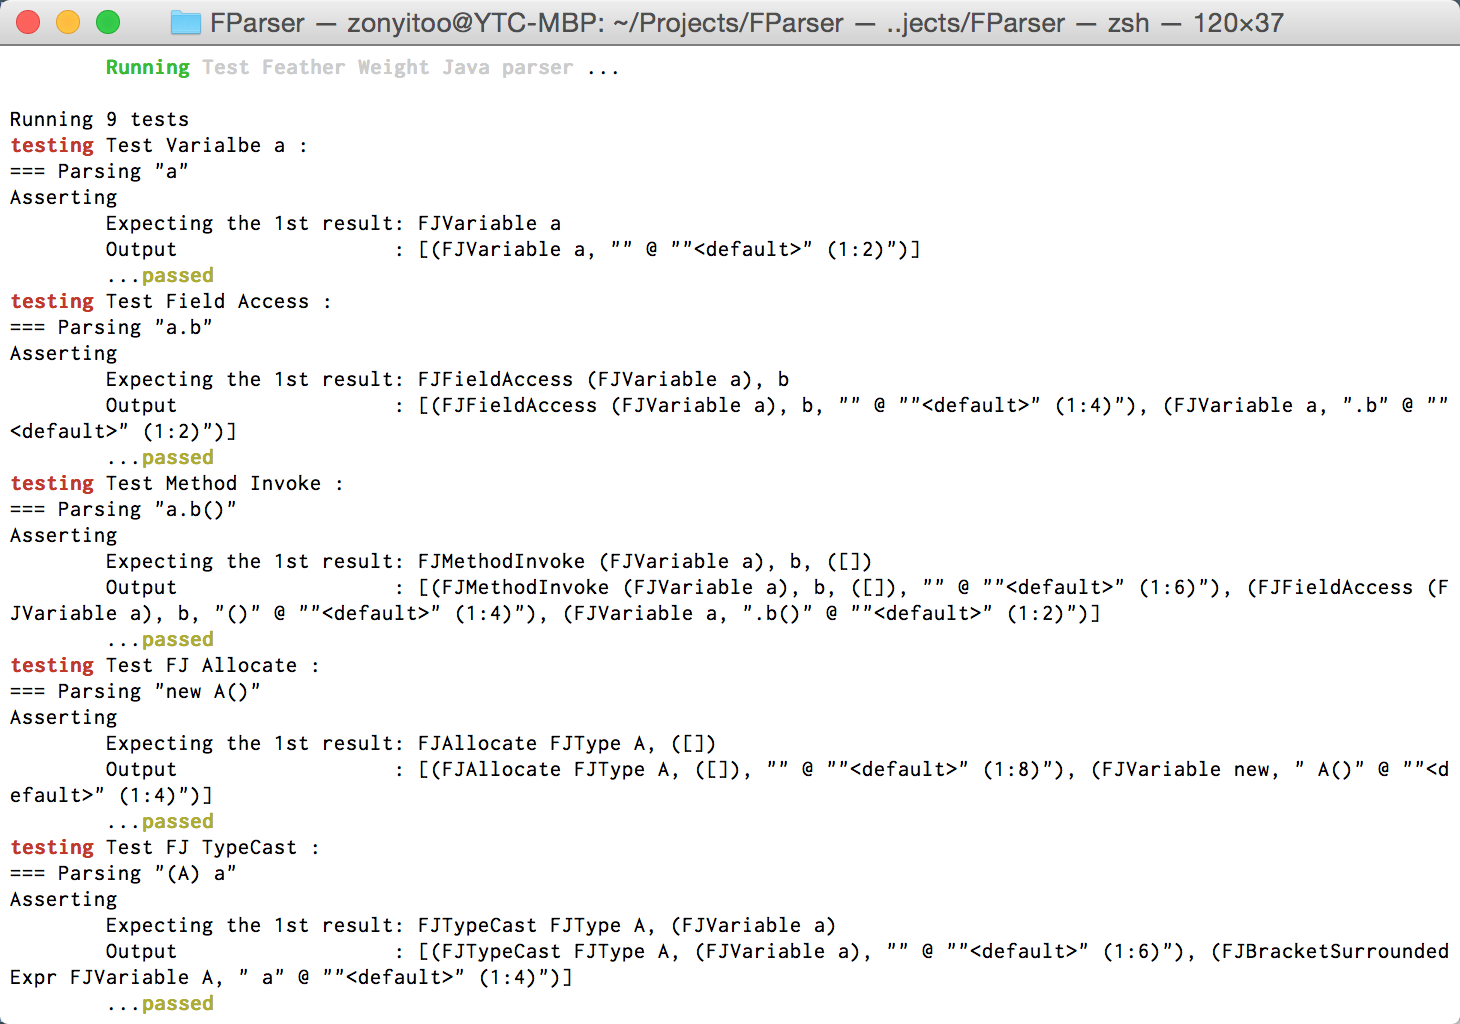
\includegraphics[width=0.8\textwidth]{imgs/Monadic_RunAllTests}
    \caption{Run all tests}
    \label{fig:monadic_runalltests}
\end{figure}
